\documentclass{beamer}
% \usepackage{pgfpages}
% \pgfpagesuselayout{4 on 1}[a4paper,landscape,border shrink=5mm]
\usepackage{tikz}
\usetikzlibrary{shapes, backgrounds, arrows, positioning}
%\usepackage{pgfplots}
\usepackage{listings}
\usepackage[utf8,latin1]{inputenc}
\usepackage[natbibapa]{apacite}
\makeatletter \def\newblock{\beamer@newblock} \makeatother  

\beamertemplatenavigationsymbolsempty
\setbeamertemplate{itemize items}[circle]
\setbeamertemplate{section in toc}[circle]
\mode<beamer>{\setbeamercolor{math text displayed}{fg=iwmgrau}}
\setbeamercolor{block body}{bg=iwmorange!50!white}
\setbeamercolor{block title}{fg=white, bg=iwmorange}

\definecolor{iwmorange}{RGB}{255,105,0}
\definecolor{iwmgrau}{RGB}{67,79,79}
\setbeamercolor{title}{fg=iwmorange}
\setbeamercolor{frametitle}{fg=iwmorange}
\setbeamercolor{structure}{fg=iwmorange}
\setbeamercolor{normal text}{fg=iwmgrau}
\setbeamercolor{author}{fg=iwmgrau}
\setbeamercolor{date}{fg=iwmgrau}

\title{Data simulation for linear mixed-effects models}
\author{Nora Umbach%\footnote{These slides are a modified version of slides created by \url{https://osf.io/ /}. }
}
%\institute{\includegraphics[scale=.15]{figures/ut_logo}}
\date{July 12, 2021}
%\date{Last modified: \today}

\newcommand{\vect}[1]{\mathbf{#1}}
\newcommand{\mat}[1]{\mathbf{#1}}
\newcommand{\gvect}[1]{\boldsymbol{#1}}
\newcommand{\gmat}[1]{\boldsymbol{#1}}

\lstset{language=R,%
  literate={Ü}{{\"U}}1
           {ü}{{\"u}}1,
  %backgroundcolor=\color{iwmgrau!80!white},
  basicstyle=\ttfamily\color{iwmorange},
  frame=single,
  commentstyle=\slshape\color{black},
  keywordstyle=\bfseries\color{white},
  identifierstyle=\color{white},
  stringstyle=\color{green!85!black},
  numbers=none,%left,numberstyle=\tiny,
  basewidth={.5em, .4em},
  showstringspaces=false,
  emphstyle=\color{red!50!white}}

\lstdefinestyle{plain}{language=R,
  frame=none,
  basicstyle=\ttfamily\color{iwmorange},
  commentstyle=\slshape\color{iwmgrau},
  keywordstyle=\bfseries\color{iwmgrau},
  identifierstyle=\color{iwmgrau},
  stringstyle=\color{iwmgrau},
  numbers=none,
  basewidth={.5em, .4em},
  showstringspaces=false}

\pgfmathdeclarefunction{gauss}{2}{%
  \pgfmathparse{1/(#2*sqrt(2*pi))*exp(-((x-#1)^2)/(2*#2^2))}%
}

\AtBeginSection[]{
  \frame{
    \tableofcontents[sectionstyle=show/hide, subsectionstyle=show/show/hide]}}

\setbeamertemplate{headline}{
 \begin{beamercolorbox}{section in head}
   \vskip5pt\insertsectionnavigationhorizontal{\paperwidth}{}{}\vskip2pt
 \end{beamercolorbox}
}

\setbeamertemplate{footline}{\vskip-2pt\hfill\insertframenumber$\;$\vskip2pt}

\begin{document}

\begin{frame}{}
\thispagestyle{empty}
\titlepage
\end{frame}

% \begin{frame}{Outline}
% \tableofcontents
% \end{frame}


\begin{frame}{Example: Crossed random effects}
  \begin{itemize}
    \item This example will show how to include subjects and items as
      crossed, independent, random effects, as opposed to hierarchical or
      multilevel models in which random effects are assumed to be nested
    \item The data are taken from \citet{Baayen2008}
    \item Assume an example data set with three participants s1, s2 and s3
      who each saw three items w1, w2, w3 in a priming lexical decision
      task under both short and long SOA conditions
    \item Let's say the data were generated by the following model
  \[
    y_{ij} = \beta_0 + \beta_1 SOA_j + \omega_{0j} + \upsilon_{0i} +
      \upsilon_{1i} SOA + \varepsilon_{ij} 
  \]
\small
with $\gvect{\upsilon} \sim N\left(\gvect{0}, \gmat{\Sigma}_{\upsilon} = 
    \begin{pmatrix}
      \sigma^2_{\upsilon_0} & \sigma_{\upsilon_0\upsilon_1} \\
      \sigma_{\upsilon_0\upsilon_1} & \sigma^2_{\upsilon_1} \\
    \end{pmatrix}\right)$,
      $\omega_{0j} \sim N(0, \sigma_{\omega}^2)$, $\varepsilon_{ij} \sim N(0,
  \sigma_{\varepsilon}^2)$, all i.i.d. 
  \end{itemize}
\end{frame}

\begin{frame}{True values}
  \begin{itemize}
    \item We assume the following true parameters for a data simulation
  \end{itemize}
  \begin{center}
  \begin{tabular}{lrr}
    \hline
    Parameter && Model \\
    \hline
    $\hat\beta_0$                     && 522.11\\
    $\hat\beta_1$                     && $-$18.89\\
    $\hat\sigma_{\omega}$             && 21.10\\
    $\hat\sigma_{\upsilon_0}$         && 23.89\\
    $\hat\sigma_{\upsilon_1}$         && 9.00\\
    $\hat\rho_{\upsilon_0\upsilon_1}$ && $-$1.00\\
    $\hat\sigma_{\varepsilon}$        && 9.90\\
    \hline
  \end{tabular}
  \end{center}
     \[
       y_{ij} = \beta_0 + \beta_1 SOA_j + \omega_{0j} + \upsilon_{0i} +
       \upsilon_{1i} SOA + \varepsilon_{ij} 
  \]
\small
with $\gvect{\upsilon} \sim N\left(\gvect{0}, \gmat{\Sigma}_{\upsilon} = 
    \begin{pmatrix}
      \sigma^2_{\upsilon_0} & \sigma_{\upsilon_0\upsilon_1} \\
      \sigma_{\upsilon_0\upsilon_1} & \sigma^2_{\upsilon_1} \\
    \end{pmatrix}\right)$,
  $\omega_{0j} \sim N(0, \sigma_{\omega}^2)$, $\varepsilon_{ij} \sim N(0,
  \sigma_{\varepsilon}^2)$ 
\end{frame}

\begin{frame}{Example data set}
  \scriptsize
With random intercepts for subject and item, and random slopes for
  subject\\[1.5ex]
  \begin{tabular}{llllcrrrcr}
    \hline
    Subj & Item & SOA & RT & Fixed &&  Random &&& Res \\
    \cline{5-6}
    \cline{7-10}
    & & & & Int & SOA & ItemInt & SubInt & SubSOA & \\
    \hline
    s1 & w1 & Long  & 466 & 522.2 & 0     & $-$28.3 & $-$26.2 & 0       & $-$2.0 \\
    s1 & w2 & Long  & 520 & 522.2 & 0     & 14.2    & $-$26.2 & 0       & 9.8 \\
    s1 & w3 & Long  & 502 & 522.2 & 0     & 14.1    & $-$26.2 & 0       & $-$8.2 \\
    s1 & w1 & Short & 475 & 522.2 & $-$19 & $-$28.3 & $-$26.2 & 11      & 15.4 \\
    s1 & w2 & Short & 494 & 522.2 & $-$19 & 14.2    & $-$26.2 & 11      & $-$8.4 \\
    s1 & w3 & Short & 490 & 522.2 & $-$19 & 14.1    & $-$26.2 & 11      & $-$11.9 \\
    s2 & w1 & Long  & 516 & 522.2 & 0     & $-$28.3 & 29.7    & 0       & $-$7.4 \\
    s2 & w2 & Long  & 566 & 522.2 & 0     & 14.2    & 29.7    & 0       & 0.1 \\
    s2 & w3 & Long  & 577 & 522.2 & 0     & 14.1    & 29.7    & 0       & 11.5 \\
    s2 & w1 & Short & 491 & 522.2 & $-$19 & $-$28.3 & 29.7    & $-$12.5 & $-$1.5 \\
    s2 & w2 & Short & 544 & 522.2 & $-$19 & 14.2    & 29.7    & $-$12.5 & 8.9 \\
    s2 & w3 & Short & 526 & 522.2 & $-$19 & 14.1    & 29.7    & $-$12.5 & $-$8.2 \\
    s3 & w1 & Long  & 484 & 522.2 & 0     & $-$28.3 & $-$3.5  & 0       & $-$6.3 \\
    s3 & w2 & Long  & 529 & 522.2 & 0     & 14.2    & $-$3.5  & 0       & $-$3.5 \\
    s3 & w3 & Long  & 539 & 522.2 & 0     & 14.1    & $-$3.5  & 0       & 6.0 \\
    s3 & w1 & Short & 470 & 522.2 & $-$19 & $-$28.3 & $-$3.5  & 1.5     & $-$2.9 \\
    s3 & w2 & Short & 511 & 522.2 & $-$19 & 14.2    & $-$3.5  & 1.5     & $-$4.6 \\
    s3 & w3 & Short & 528 & 522.2 & $-$19 & 14.1    & $-$3.5  & 1.5     & 13.2 \\
    \hline
    &&&&&& $\sigma^2_{\omega_0}$ & $\sigma^2_{\upsilon_0}$ &
    $\sigma^2_{\upsilon_1}$ & $\sigma^2_{\varepsilon}$\\ 
    &&&&&&  & \multicolumn{2}{c}{$\sigma_{\upsilon_0\upsilon_1}$} & 
  \end{tabular}
\end{frame}

{\setbeamercolor{background canvas}{bg=iwmgrau!80!white}

\begin{frame}[fragile]{Fixed effects}
  \begin{lstlisting}
datsim <- 
  expand.grid(subject = factor(c("s1", "s2", "s3")),
              item = factor(c("w1", "w2", "w3")),
              soa = factor(c("long", "short")))
datsim <- datsim[order(datsim$subject), ]

# Model matrix in dummy coding
model.matrix(~ soa, datsim)

beta0  <- 522.11
beta1  <- -18.89

b0 <- rep(beta0, 18)
b1 <- rep(rep(c(0, beta1), each=3), 3)

cbind(b0, b1)
  \end{lstlisting}
\end{frame}

\begin{frame}[fragile]{Random effects}
  \begin{lstlisting}
sw  <- 21.1
sy0 <- 23.89; sy1 <- 9; ry  <- -1
se  <- 9.9

w  <- rep(rnorm(3, mean=0, sd=sw), 6)
e  <- rnorm(18, mean=0, sd=se)
# Draw from bivariate normal dsitribution
sig <- matrix(c(sy0^2, ry*sy0*sy1, ry*sy0*sy1, sy1^2),
  2, 2)
y01 <- mvtnorm::rmvnorm(3, mean=c(0, 0), sigma=sig)
y0 <- rep(y01[,1], each=6)
y1 <- rep(c(0, y01[1,2],
            0, y01[2,2],
            0, y01[3,2]), each=3)
cbind(w, y0, y1, e)
  \end{lstlisting}
\end{frame}

\begin{frame}[fragile]{Simulate data}
  \begin{lstlisting}
datsim$rt <- b0 + b1 + w + y0 + y1 + e

# Fit model
library(lme4)

lme1 <- lmer(rt ~ soa + (1 | item) + (soa | subject),
  datsim, REML=F)
summary(lme1)
confint(lme1)

# btw
?pvalues
?convergence
  \end{lstlisting}
\end{frame}

}

\begin{frame}{Visualization of data}
  \centering
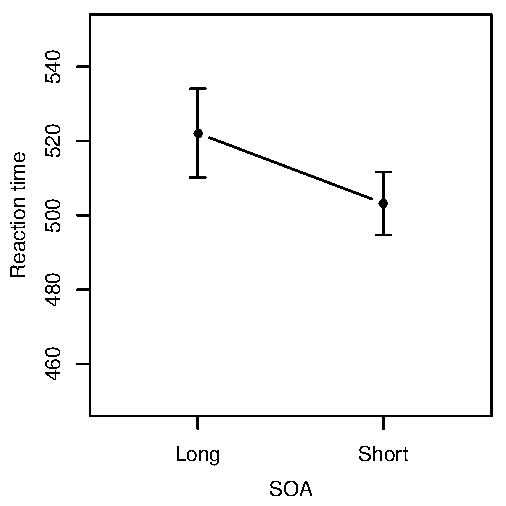
\includegraphics[scale=.8]{figures/baayen_ex_agg}
\end{frame}

\begin{frame}{Visualization of data}
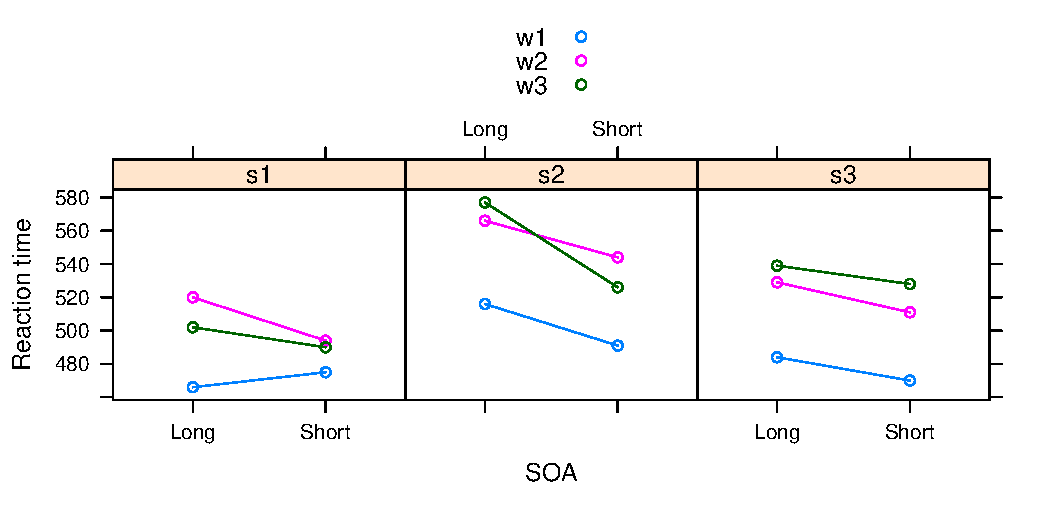
\includegraphics[scale=.65]{figures/baayen_ex}
\end{frame}

\begin{frame}{Comparison of sample and model estimates}
  For this example, we are able to compare the ``true'' values to the
  parameter estimates
  \begin{center}
  \begin{tabular}{lrrrr}
    \hline
    Parameter && Sample && Model \\
    \hline
    $\hat\beta_0$ && 522.2 && 522.11\\
    $\hat\beta_1$ && $-$19.00 && $-$18.89\\
    $\hat\sigma_{\omega}$ && 20.59 && 21.10\\
    $\hat\sigma_{\upsilon_0}$ && 23.62 && 23.89\\
    $\hat\sigma_{\upsilon_1}$ && 9.76 && 9.00\\
    $\hat\rho_{\upsilon_0\upsilon_1}$ && $-$0.71 && $-$1.00\\
    $\hat\sigma_{\varepsilon}$ && 8.55 && 9.90\\
    \hline
  \end{tabular}
  \end{center}
     \[
       y_{ij} = \beta_0 + \beta_1 SOA_j + \omega_{0j} + \upsilon_{0i} +
       \upsilon_{1i} SOA + \varepsilon_{ij} 
  \]
\small
with $\gvect{\upsilon} \sim N\left(\gvect{0}, \gmat{\Sigma}_{\upsilon} = 
    \begin{pmatrix}
      \sigma^2_{\upsilon_0} & \sigma_{\upsilon_0\upsilon_1} \\
      \sigma_{\upsilon_0\upsilon_1} & \sigma^2_{\upsilon_1} \\
    \end{pmatrix}\right)$,
  $\omega_{0j} \sim N(0, \sigma_{\omega}^2)$, $\varepsilon_{ij} \sim N(0,
  \sigma_{\varepsilon}^2)$ 
\end{frame}


\begin{frame}{Linear mixed-effects model}
  \begin{itemize}
    \item The linear mixed-effects model has the general form
\[
  \vect{y}_i = \mat{X}_i \, \gvect{\beta} + \mat{Z}_i \, \gvect{\upsilon}_i +
               \gvect{\varepsilon}_i
\]
with fixed effects $\gvect{\beta}$, random effects
$\gvect{\upsilon}_i$, and the design matrices $\mat{X}_i$ and $\mat{Z}_i$
  and the assumptions
\[
  \gvect{\upsilon}_i \sim N(\vect{0}, \, \gmat{\Sigma}_\upsilon)
    \text{ i.i.d.}, \qquad
  \gvect{\varepsilon}_i \sim N(\vect{0}, \, \sigma^2 \mat{I}_{n_i})
    \text{ i.i.d.}
\]
  \end{itemize}
\end{frame}

\begin{frame}[shrink=25]{Linear mixed-effects model}
\vspace{2cm}
\begin{equation*}
  \begin{pmatrix}
    y_1 \\
    y_2 \\
    y_3 \\
    \vdots \\
    y_N
  \end{pmatrix} = 
  \begin{pmatrix}
    1 & x_{11} & x_{12} & \dots & x_{1p} \\
    1 & x_{21} & x_{22} & \dots & x_{2p} \\
    1 & x_{31} & x_{32} & \dots & x_{3p} \\
    \vdots & \vdots & \vdots & \vdots & \vdots \\
    1 & x_{N1} & x_{N2} & \dots & x_{Np} \\
  \end{pmatrix} \cdot
  \begin{pmatrix}
    \beta_0 \\
    \beta_1 \\
    \vdots \\
    \beta_p
  \end{pmatrix} +
  \begin{pmatrix}
    z_{10} & z_{11} & \dots & z_{1q} & \dots \\
    z_{20} & z_{21} & \dots & z_{2q} & \dots \\
    z_{30} & z_{31} & \dots & z_{3q} & \dots \\
    \vdots & \vdots & \vdots & \vdots & \vdots \\
    z_{N0} & z_{N1} & \dots & z_{Nq} & \dots \\
  \end{pmatrix} \cdot
  \begin{pmatrix}
    \upsilon_{10} \\
    \vdots \\
    \upsilon_{1q}\\
    \upsilon_{20} \\
    \vdots \\
    \upsilon_{Nq}
  \end{pmatrix} + 
  \begin{pmatrix}
    \varepsilon_1 \\
    \varepsilon_2 \\
    \varepsilon_3 \\
    \vdots \\
    \varepsilon_N
  \end{pmatrix}
\end{equation*}
\end{frame}

{\setbeamercolor{background canvas}{bg=iwmgrau!80!white}

\begin{frame}[fragile]{Simulate data using model matrices}
  \begin{lstlisting}
X <- model.matrix( ~ soa, datsim)
Z <- model.matrix( ~ 0 + item + subject + subject:soa,
  datsim, contrasts.arg=list(
  subject=contrasts(datsim$subject, contrasts=FALSE)))

# Fixed effects
beta  <- c(beta0, beta1)

# Random effects
theta <- c(w = unique(w),
           y0 = y01[,1],
           y1 = y01[,2])

dat$rt2 <- X %*% beta + Z %*% theta + e
  \end{lstlisting}
\end{frame}

}


% \begin{frame}{Mixed-effects models}
%   \begin{itemize}
%     \item Mixed-effects models are a class of statistical models that
%       include fixed effects as well as random effects
%     \item Fixed effects vs.\ random effects\footnote{Some critical
%       discussion on these definitions:
%       \url{http://andrewgelman.com/2005/01/25/why_i_dont_use/}}
%     \begin{itemize}
%       \item For fixed effects, only effects of the factor levels used in the
%         present study are considered (manipulated levels, e.\,g., groups,
%         sex, \dots)\\[1ex]
% 
%         $\to$ Of interest is how these levels differ
%       \item For random effects, the factor levels considered in a study are
%         regarded as a (random) sample from some population (e.\,g., words,
%         raters, subjects, \dots)\\[1ex]
% 
%         $\to$ Of interest are conlusions about the underlying population and its
%         variation
%     \end{itemize}
%   \end{itemize}
% \end{frame}

% \begin{frame}{Data schema for dependent data}
%   \small
% \begin{columns}
%   \column{.65\textwidth}
% \begin{tabular}{cccccc}
% \hline
% Person & Time      & Observ.     & \multicolumn{3}{c}{Covariates}\\\hline
% 1      & 1         & $y_{11}$    & $x_{111}$   & \dots & $x_{11p}$  \\
% 1      & 2         & $y_{12}$    & $x_{121}$   & \dots & $x_{12p}$  \\
% .      & .         & .           & .           & \dots & .          \\
% 1      & $n_1$     & $y_{1n_1}$  & $x_{1n_11}$ & \dots & $x_{1n_1p}$\\
% .      & .         & .           & .           & \dots & .          \\
% .      & .         & .           & .           & \dots & .          \\
% $N$    & 1         & $y_{N1}$    & $x_{N11}$   & \dots & $x_{N1p}$  \\
% $N$    & 2         & $y_{N2}$    & $x_{N21}$   & \dots & $x_{N2p}$  \\
% .      & .         & .           & .           & \dots & .          \\
% $N$    & $n_N$     & $y_{Nn_N}$  & $x_{Nn_N1}$ & \dots & $x_{Nn_Np}$\\
% \hline
% \end{tabular}
% %
%   \column{.45\textwidth}
% \begin{itemize}
% \item $i = 1, \dots, N$ persons
% \item $j = 1, \dots, n_i$ time points for person $i$
% \item All observations: $\sum_i^N n_i$
% \item Vector of all observations for person $i$\\
%   $(\vect{y}_i)_{n_i \times 1}$\\
% \item Vector of covariates for person $i$ at time point $j$\\
%   $(\vect{x}_{ij})_{p \times 1}$
% \item All covariates of person $i$\\
%   $(\vect{X}_i)_{n_i \times p}$
% \end{itemize}
% \end{columns}
% \end{frame}

% \begin{frame}[fragile]{Structure of data}
%   \begin{lstlisting}
% > xtabs( ~ Subject + Days, sleepstudy)
%        Days
% Subject 0 1 2 3 4 5 6 7 8 9
%     308 1 1 1 1 1 1 1 1 1 1
%     309 1 1 1 1 1 1 1 1 1 1
%     310 1 1 1 1 1 1 1 1 1 1
%     330 1 1 1 1 1 1 1 1 1 1
%     331 1 1 1 1 1 1 1 1 1 1
%     332 1 1 1 1 1 1 1 1 1 1
%     333 1 1 1 1 1 1 1 1 1 1
%     334 1 1 1 1 1 1 1 1 1 1
%     335 1 1 1 1 1 1 1 1 1 1
%     337 1 1 1 1 1 1 1 1 1 1
%     349 1 1 1 1 1 1 1 1 1 1
%     350 1 1 1 1 1 1 1 1 1 1
%     351 1 1 1 1 1 1 1 1 1 1
%     ...
%   \end{lstlisting}
% \end{frame}

% {\setbeamercolor{background canvas}{bg=iwmgrau!80!white}
% 
% \begin{frame}[fragile]{}
%   \begin{lstlisting}
%   ##
%   \end{lstlisting}
% \end{frame}
% 
% }
% 
% \begin{frame}[fragile]{}
%   \begin{block}{Exercise}
%     \begin{itemize}
%       \item 
%     \end{itemize}
%   \end{block}
% \end{frame}

\appendix
%\begin{frame}[allowframebreaks]{References}
\begin{frame}{References}
%\renewcommand{\bibfont}{\footnotesize}
\bibliographystyle{apacite}
\bibliography{../../../literature/nu}
\vfill
\end{frame}

\end{document}

